\subsection{Απάντηση Υποερωτήματος (α)}
\label{ssec:Solution_1.1}
\doublespacing
Η μηχανή μας λοιπόν παίρνει μία λέξη συμπεριλαμβανομένης της κενής ανάμεσα σε δύο κενά και ουσιαστικά κάνει δύο
πράγματα:
\begin{itemize}
	\itemsep0em
	\item Αντιγραφή της αμέσως στα δεξιά της (και άρα προώθηση του κενού κατά $|w|$ θέσεις
	\item Αναστροφή της αρχικής λέξης επί της ιδίας θέσης που αυτή κατείχε.
	\item Επιπροσθέτως εμείς θα προσθέσουμε έλεγχο για κενή λέξη απευθείας στην εκκίνηση από τη μία για να
	αποφύγουμε περιττές διαδικασίες σε αυτή τη περίπτωση, από την άλλη διότι το αυτόματο μας θα πρέπει να μην
	μπορεί να περιέλθει σε κάποια ασαφή κατάσταση, από την οποία να μην μπορεί να διαφύγει έτσι ώστε να τερματίσει.
\end{itemize}

\par Ο τρόπος που σκεφθήκαμε εν προκειμένω για την επίλυση του συγκεκριμένου προβλήματος και άρα η σχεδίαση που θα
δώσουμε έχει ως εξής:
\begin{itemize}
	\itemsep0em
	\item Αρχικά θα χρησιμοποιήσουμε τεχνική "διαίρει και βασίλευε" για να αποσυνθέσουμε το πρόβλημα σε απλούστερα
	που το αποτελούν.
	\item Το κάθε ένα από αυτά τα προβλήματα θα έχουν τη δική τους μηχανή Turing που θα τα επιλύει.
	\item Η τελική μηχανή θα κατασκευάζεται από σειριακή (με πιθανή διακλάδωση) συνένωση αυτών των επιμέρους
	μηχανών.\clearpage
	\item Οι επιμέρους μηχανές υποθετικά έχουν ως εξής (αργότερα ίσως δούμε ότι ίσως χρειαστούμε λιγότερες ή
	περισσότερες):
		\begin{enumerate}
			\item $M_1:$ Έλεγχος για κενή ή μη λέξη.

			\item $Μ_2:$ Αντιγραφή λέξης.

			\item $Μ_3:$ Αναστροφή λέξης

			\item $M_4:$ Μετακίνηση στη τελική θέση που απαιτούν οι προδιαγραφές να βρεθεί η κεφαλή της μηχανής.
		\end{enumerate}
\end{itemize}

\par Είμαστε έτοιμοι για την κατασκευή των επιμέρους μηχανών. Για λόγους ευκολίας θα τις διατυπώσουμε πρόχειρα με
ιδιότυπο μαθηματικό συμβολισμό για διευκόλυνση μας:

\par Η μηχανή $M_1$ θέλουμε απλά να ελέγχει αν η $w$ είναι κενή και αν ναι να μετακινεί την
κεφαλή στη πρώτη θέση μετά την αρχή της ταινίας, η οποία θέση θα πρέπει απαραίτητα να είναι κενή.
Αυτό το πετυχαίνει κάνοντας μία μετακίνηση δεξιά ώστε να βρεθεί η κεφαλή εκεί που αναμένετε (υποχρεωτικά) το πρώτο σύμβολο
της λέξης και κατόπιν ελέγχει εάν αυτό όντως ανήκει στα σύμβολα της λέξης ή όχι (άρα κενό) και δρομολογεί ανάλογα στην
αντίστοιχη επόμενη μηχανή.
\[\text{Έλεγχος κενής λέξης}\,:\, M_1\,:\quad M_4\,\overset{\sqcup}{\longleftarrow}\overset{\lor}{{\text{\large\bfseries
R}}}\overset{x \in \{a,\,b\}}{\longrightarrow}\, M_2\]
\par Δοκιμή:
\begin{itemize}
	\itemsep0em
	\item $|w| = 0 \;\Rightarrow\;\triangleright\, \underline{\sqcup}\, \sqcup \xrightarrow{R}
	 		\triangleright\, \sqcup\, \underline{\sqcup} \xrightarrow{\sqcup} M_4 \quad$ \textcolor{green}{\ding{51}}

	\item $|w| = n, n \geq 1 \;\Rightarrow\;\triangleright\, \underline{\sqcup}\, w_1\,...\,w_n \sqcup \xrightarrow{R}
	\triangleright\, \sqcup\, \underline{w_1}\,...\,w_n\, \sqcup \xrightarrow{x \in \{a,\,b\}} M_2 \quad$
	\textcolor{green}{\ding{51}}
\end{itemize}

\par Η μηχανή $M_2$ έχει ως αποστολή την αντιγραφή συμβολοσειράς $w$ δεξιά της ιδίας αρχικής $w$.
Στην δική μας επίλυση τοποθετούμε βοηθητικό κενό ανάμεσα ως δείκτη, όπου θα αφαιρεθεί από την μηχανή $M_3$.
Ενδεχομένως η συγκεκριμένη λύση να επιδέχεται βελτιστοποίησης αλλά θεωρούμε ότι είναι επαρκέστατη.
\[\text{Αντιγραφή λέξης}\,:\, M_2\,:\quad M_3\, \xleftarrow{\sqcup}\overset{\lor}{\text{\large\bfseries\$}}\,R^2_\sqcup
\,x\,L_\$\,R\,\xrightarrow{x\in\{a,\,b\}}\, M_2\]
\par Δοκιμή:
\begin{itemize}
	\itemsep0em
	\item $w = abb \;\xRightarrow{M_1}\;\triangleright\, \sqcup\, \underline{a}\, b\,b\, \sqcup\, \xrightarrow{\$}\,
	\triangleright\, \sqcup\, \underline{\$}\, b\,b\, \sqcup\, \xrightarrow{R^2_\sqcup}\,
	\triangleright\, \sqcup\, \$\, b\,b\, \sqcup\, \underline{\sqcup}\, \xrightarrow{x}\,
	\triangleright\, \sqcup\, \$\, b\,b\, \sqcup\, \underline{a}\\ \xrightarrow{L_\$}
	\triangleright\, \sqcup\, \underline{\$}\, b\,b\, \sqcup\, a\, \xrightarrow{R}\,
	\triangleright\, \sqcup\, \$\, \underline{b}\,b\, \sqcup\, a\,
	\xrightarrow{x\in\{a,\,b\}}\, M_2\, \xrightarrow{\$\, R^2_\sqcup\, x\, L_\$\, R}\,
	\triangleright\, \sqcup\, \$\, \$\,\underline{b}\, \sqcup\, a\,b\, \\
	\xrightarrow{x\in\{a,\,b\}}\, M_2\, \xrightarrow{\$\,R^2_\sqcup\, x\, L_\$\, R}\,
	\triangleright\, \sqcup\, \$\, \$\,\$\, \underline{\sqcup}\, a\,b\,b\,
	\xrightarrow{\sqcup} M_3\,
	    \quad$
	\textcolor{green}{\ding{51}}
\end{itemize}


\par Ακολουθεί μηχανή $M_3$ οποία έχει ως σκοπό αναστροφή αρχικής λέξης. Αρχικά όπως το είχαμε σκεφθεί εκτελούσε
μόνο αυτό το σκοπό, αφήνοντας σε επόμενη μηχανή την αφαίρεση του ενδιάμεσου κενού. Αργότερα ερευνήσαμε αν γίνεται να
γίνουν και τα δύο σε μία λειτουργία, χωρίς όμως ουσιαστικά να γίνει ο τοπικός αλγόριθμος πιο περίπλοκος έτσι ώστε να
μειώσουμε την στρατηγική περιπλοκότητα. Εν τέλη βρέθηκε μηχανή που κάνει ακριβώς αυτό, ελαχιστοποιώντας αυτές τις δύο
διαδικασίες ενώ παραμένει απλό και κατανοητό. Με αυτό τον τρόπο επίσης μειώνονται και οι περιττές μετακινήσεις της κεφαλής
έτσι ώστε αν αυτό το θεωρητικό μοντέλο αποκτούσε φυσική υλοποίηση, ο όλος μηχανισμός να δεχόταν λιγότερες καταπονήσεις
(παρόλο που δεν αφορά το ερώτημα).
\[\text{Αναστροφή αρχικής λέξης και αφαίρεση ενδιάμεσου κενού}\,:\, M_3\,:\]
\[M_4 \xleftarrow{\sqcup}\,\overset{\lor}{{\text{\large\bfseries R}}}\,\xrightarrow{x\in\{a,\,b\}}\,
	\sqcup\, L\, x\, L_\$\,x\, R_\sqcup\, \rightarrow\, M_3\]
\par Δοκιμή:
\begin{itemize}
	\itemsep0em
	\item $w = abb \;\xRightarrow{M_2}\;
	\triangleright\, \sqcup\, \$\, \$\,\$\, \underline{\sqcup}\, a\,b\,b\, \xrightarrow{R}\,
	\triangleright\, \sqcup\, \$\, \$\,\$\, \sqcup\, \underline{a}\,b\,b\, \xrightarrow{\xrightarrow{x\in\{a\,b\}}\sqcup}\\
	\triangleright\, \sqcup\, \$\, \$\,\$\, \sqcup\, \underline{\sqcup}\,b\,b\, \xrightarrow{L}\,
	\triangleright\, \sqcup\, \$\, \$\,\$\, \underline{\sqcup}\, \sqcup\,b\,b\, \xrightarrow{x}\,
	\triangleright\, \sqcup\, \$\, \$\,\$\, \underline{a}\, \sqcup\,b\,b\, \xrightarrow{L_\$}\\
	\triangleright\, \sqcup\, \$\, \$\,\underline{\$}\, a\, \sqcup\,b\,b\, \xrightarrow{x}\,
	\triangleright\, \sqcup\, \$\, \$\,\underline{a}\, a\, \sqcup\,b\,b\, \xrightarrow{R_\sqcup}\,
	\triangleright\, \sqcup\, \$\, \$\,a\, a\, \underline{\sqcup}\,b\,b\, \xrightarrow{}\, M_3\\
	\xrightarrow{R}\,
	\triangleright\, \sqcup\, \$\, \$\,a\, a\, \sqcup\,\underline{b}\,b\, \xrightarrow{\xrightarrow{x\in\{a\,b\}}\sqcup}
	\triangleright\, \sqcup\, \$\, \$\,a\, a\, \sqcup\,\underline{\sqcup}\,b\,
	\xrightarrow{\sqcup\,L\,x\,L_\$\,x\,R_\sqcup}\\
	\triangleright\, \sqcup\, \$\, b\,a\, a\, \,b \,\underline{\sqcup}\,b \,\xrightarrow{} \,M_3\, \xrightarrow{R}\,
	\triangleright\, \sqcup\, \$\, b\,a\, a\, \,b \,\sqcup\,\underline{b}\, \xrightarrow{\xrightarrow{x\in\{a\,b\}}\sqcup}
	\triangleright\, \sqcup\, \$\, b\,a\, a\, \,b \,\sqcup\,\underline{\sqcup}\\
	\xrightarrow{\sqcup\,L\,x\,L_\$\,x\,R_\sqcup}
	\triangleright\, \sqcup\, b\, b\,a\, a\, \,b \,b\,\underline{\sqcup}\, \xrightarrow{}\, M_3 \xrightarrow{R}\,
	\triangleright\, \sqcup\, b\, b\,a\, a\, \,b \,b\,\sqcup\,\underline{\sqcup}\,
	\xrightarrow{\sqcup} M_4 \quad$ \textcolor{green}{\ding{51}}
\end{itemize}

\par \par Τέλος έχουμε τη μηχανή $M_4$ με μοναδικό σκοπό την επαναφορά της κεφαλής στο αριστερότατο κενό κατά τις
προδιαγραφές που μας έχουν δοθεί.
\[\text{Μετακίνηση κεφαλής στο αριστερότατο κενό}\,:\, M_4\,:\]
\[\overset{\lor}{{\text{\large\bfseries L}}}_\triangleright\, R\]
\par Δοκιμή:
\begin{itemize}
	\itemsep0em
	\item $w = abb \;\xRightarrow{M_3}\;
	\triangleright\, \sqcup\, b\, b\,a\, a\, \,b \,b\,\sqcup\,\underline{\sqcup}\, \xrightarrow{L_\triangleright}\,
	\underline{\triangleright}\, \sqcup\, b\, b\,a\, a\, \,b \,b\,\sqcup\,\sqcup\, \xrightarrow{R}\\
	\triangleright\, \underline{\sqcup}\, b\, b\,a\, a\, \,b \,b\,\sqcup\,\sqcup\,\quad$ \textcolor{green}{\ding{51}}

	\item $|w| =0 \;\xRightarrow{M_1}\;
	\triangleright\, \sqcup\, \underline{\sqcup} \xrightarrow{L_\triangleright}\,
	\underline{\triangleright}\, \sqcup\, \sqcup \xrightarrow{R} \triangleright\, \underline{\sqcup}\, \sqcup \quad$
	\textcolor{green}{\ding{51}}
\end{itemize}

\par Σχεδιάζουμε γραφικά τη διασύνδεση των μηχανών μεταξύ τους και κατόπιν επανασχεδιάζουμε αντικαθιστώντας τες με τα
αντίστοιχα διαγράμματα εσωτερικής λειτουργίας τους, έτσι ώστε να καταλήξουμε στην ζητούμενη μηχανή.


\begin{center}
	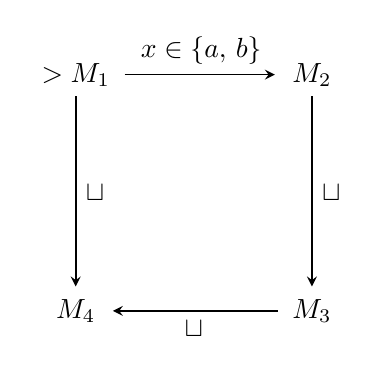
\begin{tikzpicture}[->,>=stealth, shorten >=1pt,semithick,node distance=3.0cm,auto]

		\node(q_1)                  {$\,>M_1\,$};
		\node(q_2) [right of = q_1] {$\,M_2\,$};
		\node(q_3) [below of = q_2] {$\,M_3\,$};
		\node(q_4) [below of = q_1] {$\,M_4\,$};

		\draw[->] (q_1) -- node {$x\in\{a,\,b\}$} (q_2);
		\draw[->] (q_2) -- node {$\sqcup$} (q_3);
		\draw[->] (q_3) -- node {$\sqcup$} (q_4);
		\draw[->] (q_1) -- node {$\sqcup$} (q_4);
	\end{tikzpicture}
	\vspace{-0.3cm}
\end{center}


\begin{tcolorbox}[colback=yellow!15!white, colframe=blue!50!white,
	fonttitle=\bfseries\Large, title = Γραφική αναπαράσταση τελικής πρότυπης μηχανής Turing]

\begin{center}
	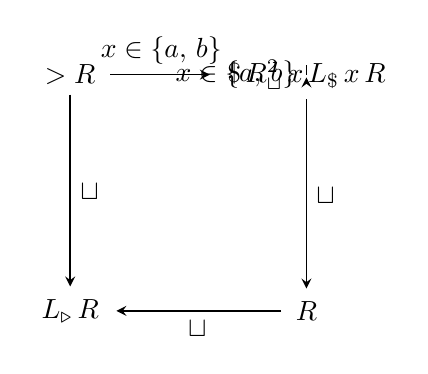
\begin{tikzpicture}[->,>=stealth, shorten >=1pt,semithick,node distance=3.0cm,auto]

		\node(q_1)                  {$\,>R\,$};
		\node(q_2) [right of = q_1] {$\,\$\,R^2_\sqcup\,x\,L_\$\,x\,R\,$};
		\node(q_3) [below of = q_2] {$\,R\,$};
		\node(q_4) [below of = q_1] {$\,L_\triangleright\,R\,$};

		\draw[->] (q_1) -- node {$x\in\{a,\,b\}$} (q_2);
		\draw[->] (q_1) -- node {$\sqcup$} (q_4);
		\draw[->] (q_2) -- node {$x\in\{a,\,b\}$} (q_2);
		\draw[->] (q_2) -- node {$\sqcup$} (q_3);
		\draw[->] (q_3) -- node {$\sqcup$} (q_4);
	\end{tikzpicture}
	\vspace{-0.3cm}
\end{center}

\end{tcolorbox}



\begin{center}
	%\vspace{2em}
	\noindent\rule{\linewidth}{0.5pt}
	%\vspace{2em}
\end{center}
%\clearpage